\documentclass{article}

\usepackage[utf8]{inputenc}  
\usepackage[T1]{fontenc}   
\usepackage{amsmath}
\usepackage{amsfonts}
\usepackage{pgfplots}
\usepackage{sagetex}
\usepackage{graphicx}
\usepackage{caption}
\usepackage{subcaption}

\usepackage{geometry}
\geometry{hmargin=1.5cm,vmargin=1.5cm}

\newcommand{\BigO}[1]{\ensuremath{\operatorname{O}\left(#1\right)}}
\newcommand{\SmallO}[1]{\ensuremath{\operatorname{o}\left(#1\right)}}

\newcommand{\BBigO}[3]{\ensuremath{\underset{#1 \to #2 }{\operatorname{O}\left(#3\right)}}}
\newcommand{\BigF}[2]{\ensuremath{#1 \left(#2\right)}}
\newcommand{\Wrap}[1]{\ensuremath{\left(#1\right)}}
\newcommand{\Q}[1]{\subsubsection*{Question #1}}
\newcommand\Coord[2]{\ensuremath{\begin{pmatrix}
 #1 \\
 #2 
\end{pmatrix}}}
\def\FunctionQ(#1, #2, #3){
\addplot[color= #3,samples=100,domain=0.01:0.6] 
{ rad(asin(#1 * sin(deg(pi * #2))))/(#1 * pi * #2) };
\addlegendentry{$\alpha = #1$}

}

\def\FunctionP(#1, #2, #3, #4){
\addplot[color= #4,samples=100,domain=0.01:0.6] 
{ rad(asin(#1 * sqrt( (sin(deg(pi * #2 * cos(deg(#3))))^2  + (sin(deg(pi * #2 * sin(deg(#3)))))^2 ))/(#1 * pi * #2) };
\addlegendentry{$\alpha = #1, \theta=#3$}

}

\begin{document}

\title{MAP431 - Devoir à la maison}
\author{EL KHADIR Bachir}


\maketitle

\Q{1} 
Soit $u(x,t) = exp\,i(w(k)t-kx)$ une solution harmonique de l'équation des ondes (1), alors:
$$ 0 = \frac{1}{c^2} \frac{\partial^2{u}}{\partial{t^2}} - \frac{\partial^2{u}}{\partial{x^2}} 
= [\frac{1}{c^2} (iw(k))^2 - (-ik)^2 ]exp\,i(w(k)t-kx)$$
d'où: $$\frac{w(k)^2}{c^2}= k^2$$
et:
$$ \lambda = \frac{2\pi}{|k|} = \frac{2 \pi c}{|w(k)|} = c T $$

Chaque signal régulier se décompose par Fourier en une somme d'ondes plane harmonique. 
On vient de montrer que toutes ces composantes ont la même vitesse de phase 
$ V = \frac{w}{k} = c$.

Le signal se propage donc sans se déformer si le milieu est homogène.

% -------------------------------------------- QUESTION 2 --------------------------------------------
\Q{2}

On suppose maintenant que les donnés initiales sont $D$-périodiques.

Si $u(x,t) = exp\,i(wt-kx)$ une solution, alors $u(0,0)=u(D,0)$.
ie $1 = expt(-ikD)$, 
ie il existe un $L \in \mathbb{Z}$ tel que $$kD = 2\pi L$$

Appliquons la transformée de Fourier discrête au problème $(1)$, il devient:

\[
\left\{
\begin{array}{r c l}
\frac{1}{c^2} \frac{\partial^2 \hat{u} }{\partial t^2} + k^2 \hat{u} & = &0 \\
\hat{u}(k, 0) & = & \hat{u_0}(k) \\
\frac{ \partial \hat{u} }{\partial t} & = & \hat{u}_1(k)
\end{array}
\right.
\]

De solution 
$$ \hat{u}(k, t) =  \hat{u}_0(k) cos(kc t) + \frac{\hat{u}_1(k)}{kc} sin(kc t)  $$
Pour $k = k_L$ , les ondes planes harmoniques sont donc détérminées par:
$$ \hat{u}_L(t) = \hat{u}(k_L,t)  = \hat{u}_{0, L} cos(w_L t) + \hat{u}_{1, L} sinc(w_L t) t$$

\begin{comment}
Réciproquement, une onde plane harmonique dont $w$ et $k$ vérifient la relation de dispersion et la relation précédente est solution du problème $(1)$.\\
Les solutions du problèmes de la forme $(2)$ sont donc:
$$ \hat{u}^+_L(t) = exp ( i\,w_L t) \, e^{-i k_L x} = [ cos(w_L t) + i w_L sinc(w_L t) t] e^{-i k_L x} $$
et 
$$ \hat{u}^-_L(t) = exp ( -i\,w_L t) \, e^{-i k_L x} = [ cos(w_L t) - i w_L sinc(w_L t) t] e^{-i k_L x} $$

Comme les vecteurs \Coord{1}{1} et \Coord{1}{-1} forment un base de $\mathbb{R}^2$, 
les combinaisons linéaires de $\hat{u}^+_L$ et de $\hat{u}^-_L$ génèrent
toutes les fonctions du type:
$$ \hat{u}_L(t) = [ \hat{u}_{0, L} cos(w_L t) + \hat{u}_{1, L} sinc(w_L t) t] e^{-i k_L x} $$

Comme le problème est linéaire, chaque $\hat{u}_L(t)$ est une solution.
\end{comment}
 Elle est associée aux conditions initiales suivantes:
$$ u_L(x, 0) = \hat{u}_{0,L} e^{-i k_L x} $$
$$ \frac{ \partial u_L }{ \partial t }(x, 0) = \hat{u}_{1,L} e^{-i k_L x} $$

La relation de dispersion étant:
$$\frac{w_L^2}{c^2}= k_L^2$$

Les fréquences spatiales sont $ \frac{1}{ \lambda } = \frac{k}{2 \pi } = \frac{L}{D}$. Elles sont inversement proportionnelles à $D$.

% -------------------------------------------- QUESTION 3 --------------------------------------------
\Q{3}
\subsubsection*{Relation de dispersion:}

Pour la fonction $U_h(k)$, on trouve:
$$ \frac{\mathrm{d}^2 U_j} {\mathrm{d}t^2} = -w(k)^2 U_j(t) $$
$$ U_{j+1} - 2U_j + U{j-1} = (exp(-ikh)  - 2 + exp(ikh)) U_j = 2(cos(kh)-1) U_j = -4sin^2 \frac{kh}{2} U_j $$
En appliquant le schéma (4): 
$$ 0 = -\frac{w(k)^2}{c^2} U_j + 4\frac{sin^2 \frac{kh}{2} }{h^2} U_j$$
donc 
$$ w(k)^2 = 4\frac{c^2}{h^2}sin^2 \frac{kh}{2} $$
donc
$$ w = \pm w_h(k), \ w_h(k) = \frac{2c}{h}sin \frac{kh}{2}$$

Cette fois la vitesse de propagation des différentes composantes de Fourrier $ V = C\,sinc \frac{kh}{2}$ dépend de la longueur d'onde $k$, la distance entre le signal calculé numériquement et le signal original augmente au cours du temps.

\subsubsection*{Control de la déformation:}

Pour tout $x \ge 0$, on a: $x - \frac{x^3}{3} \leq sin(x) \leq x$, 

donc $$-\frac{x^2}{3} \leq \frac{sin(x)}{x} - 1 \leq 0 $$
$$ |sinc(x) - 1| \leq \frac{x^2}{3}$$
pour $x = \frac{kh}{2}$ on trouve le résultat $$ |sinc(\frac{kh}{2}) - 1| \leq \frac{x^2}{3}$$

\subsubsection*{La forme de la solution:}
Comme dans la question 2, en passant à Fourier discrêt dans $(4)$, on trouve:
$$ \frac{\mathrm{d}^2 \hat{U_h} } {\mathrm{d}t^2} + \frac{4 c^2 \, sin^2\frac{kh}{2}}{h^2} \hat{U_h} = 0$$
qui donne compte tenu de la formule de dispersion:
$$ \frac{\mathrm{d}^2 \hat{U_h} } {\mathrm{d}t^2} + w_h(k)^2 \hat{U_h} = 0$$

qui a pour solution pour $k = k_L$:
$$ \hat{U_h}(t) = \hat{u}_{0, L} cos(w_{L,h}t) + \hat{u}_{1, L} sinc(w_{L, h} t) t $$
qui est associée aux conditions intiales:
$$ U_h(0) = \hat{u}_{0, L} e^{-ik_L X_h}$$
et 
$$ \frac{\mathrm{d}U_h}{\mathrm{d}t}(0) = \hat{u}_{0, L} e^{-ik_L X_h}$$

Le schéma est donc d'odre 2. En effet:
$$ w_{L,h} = \frac{2c}{h} sin \frac{k_L h}{2} = \frac{2c}{h} \left( \frac{k_L h}{2} + \BigO{h^3} \right) = ck_L + \BigO {h^2} = w_L + \BigO {h^2}$$

Notons $ f(L) = sin^2 \frac{k_L h}{2} = sin^2 \frac{2\pi L h}{2 D}$. On a:
$$ f(L + J) = \BigF{sin^2} {\frac{2\pi L  h}{2 D} + \frac{2\pi J  h}{2 D}} = \BigF{sin^2}{\frac{2\pi L  h}{2 D} + \pi } = f(L) $$
$f$ est donc périodique. 

De la relation de dispersion, $w_{L,h}$ est aussi périodiqie en $L$. Il convient donc de ne s'intéresser qu'aux $J$ premiers modes de Fourier.

$$ q_h(G) = \frac{w_h}{kc} = \frac{ \frac{2c}{h} sin \frac{kh}{2} } {kc}  = sinc \frac{kh}{2} = sinc(\pi G) $$

\begin{center}
\begin{tikzpicture} 
\begin{axis}[
xlabel=$G$,
ylabel={$q_h(G)$}
]

\addplot[samples=500,domain=0.01:0.6] {sin(deg(pi*x)) / (pi*x) };
\end{axis}
\end{tikzpicture}
\end{center}

Pour le cas périodique, on a $2 \pi L = k D = k J h$. Donc:
$$ G = \frac{k h}{2 \pi} = \frac{L}{J}$$

% -------------------------------------------- QUESTION 4 --------------------------------------------
\Q{ 4}
Le schéma est explicite. En effet, de l'expression:
$$ \frac{1}{c^2} \frac{U^{n+1}_{j} - 2U^{n}_{j} + U^{n-1}_{j}}{\Delta t^2} - \frac{U^{n}_{j+1} - 2U^{n}_{j}+U^{n}_{j-1}}{h^2} = 0 $$
On déduit que:
\begin{align*}
	U^{n+1}_{j} &= 2 U^{n}_{j} - U^{n-1}_{j} + \frac{c^2 \Delta t^2 }{h^2} \Wrap( U^{n}_{j+1} - 2U^{n}_{j}+U^{n}_{j-1}) \\
							&= \alpha ^ 2 U^{n}_{j+1} + 2(1-\alpha ^2) U^{n}_{j} + \alpha ^2 U^{n}_{j-1} - U^{n-1}_{j}
\end{align*}

Où $ \alpha = \frac{c}{\frac{h}{ \Delta t }}$ est le rapport entre le pas de progression en temps $c \Delta t$ et en espace $h$ du schéma numérique. La stabilité de ce dernier dépendra de sa valeur.


% -------------------------------------------- QUESTION 5 --------------------------------------------
\Q{5}
Pour $ 1 \leq j \leq J$ on a:
\begin{align*}
u(x_j, \Delta t) 
&= u(0,x_j) + \Delta t \, \frac{\partial u}{\partial t} (0, x_j)  + \frac{\Delta t^2}{2} \frac{\partial^2 u}{\partial t^2} (0, x_j) +  \BigO{\Delta t^3} \\
&= U_{0,j} + \Delta t U_{1,h} + \frac{\Delta t^2}{2} \frac{\partial^2 u}{\partial t^2} (0, x_j) + \BigO{\Delta t^3} 
\end{align*}
Donc $ U_{0,j} + \Delta t \, U_{1,h} $ est une approximation en temps d'ordre 1 uniquement.

$$\left( (I - \frac{c^2 \Delta t^2}{2} A_h ) U^0_h + \Delta t \, U_{1,h} \right )_j 
= u(0, x_j) - (u(x_{j+1}, 0) - 2 u(x_j, 0) + u(x_{j-1}, 0))\frac{c^2 \Delta t^2}{2 h^2} + \Delta t \frac{\partial u}{\partial t} (0, x_j) \\
$$
Mais comme $u(x_{j+1}, 0) - 2 u(x_j, 0) + u(x_{j-1}, 0) = h^2 \frac{\partial^2 u}{\partial x^2} (0, x_j) + \BigO{ h^3}$, alors:

\begin{align*}
\left( (I - \frac{c^2 \Delta t^2}{2} A_h ) U^0_h + \Delta t \, U_{1,h} \right )_j &=
u(0, x_j) - \frac{c^2 \Delta t^2}{2} \frac{\partial^2 u}{\partial x^2}  + \Delta t \frac{\partial u}{\partial t} + \BBigO{h}{0}{1} \, \BBigO{\Delta t}{0}{\Delta t^3} \\
&= u(0, x_j) - \frac{\Delta t^2}{2} \frac{\partial^2 u}{\partial t^2}  + \Delta t \frac{\partial u}{\partial t}  +  \BigO{\Delta t^3} \\
&= u(\Delta t, x_j) + \BigO{\Delta t^2}
\end {align*}

C'est donc bien un schéma d'odre 2.

% -------------------------------------------- QUESTION 6 --------------------------------------------
\Q{6}
Pour la solution particulière $U^n_h$, le schéma donne:
$$ \frac{1}{c^2} \frac{U^{n+1}_{j} - 2U^{n}_{j} + U^{n-1}_{j}}{\Delta t^2} = \frac{U^{n}_{j+1} - 2U^{n}_{j}+U^{n}_{j-1}}{h^2}$$

ie:
$$ \frac{1}{c^2} \frac{e^{i w_{h, \Delta t} (k) t} - 2 + e^{-i w_{h, \Delta t} (k) t}}{\Delta t^2} U^n_j 
= \frac{e^{-ikh} - 2+e^{ikh}}{h^2} U^n_j $$

ie:
$$  \frac{1}{c^2} \frac{-2( 1 - cos(i w_{h, \Delta t} (k) t))}{\Delta t^2} 
= \frac{-2(1-cos(kh))}{h^2}  $$

ie:
$$ \frac{4}{\Delta t^2} sin^2 \frac{w_{h, \Delta t} (k) t}{2} = \frac{4c^2}{h^2} sin^2 \frac{kh}{2} $$

ou encore:
$$ sin^2 \frac{w_{h, \Delta t} (k) t}{2} = \alpha ^ 2 sin^2 \frac{kh}{2} $$

Si $\alpha > 1$ le schéma est instable. 
En effet, pour les valeurs de $h$ et $k$ telles que $\frac{kh}{2} \approx \frac{\pi}{2}\,[2 \pi]$, on a:
$$ sin^2 \frac{w_{h, \Delta t} (k) \Delta t}{2} \approx \alpha ^ 2 > 1 $$
Ce qui est absurde.

\subsubsection*{Forme de la solution:}

\textbf{$ \alpha < 1$}

Appliquons la transofrmée de Fourier discrète à la relation explicite trouvée à la question 4:
	$$U^{n+1}_{j} = \alpha ^ 2 U^{n}_{j+1} + 2(1-\alpha ^2) U^{n}_{j} + \alpha ^2 U^{n}_{j-1} - U^{n-1}_{j} $$
On trouve:
\begin{align*}
	\hat{U}^{n+1}_{L,h} &= \alpha ^ 2 \hat{U}^{n}_{L,h}\,e^{-ihk} + 2(1-\alpha ^2) \hat{U}^{n}_{L,h} + \alpha ^2 \hat{U}^{n}_{h}\,e^{ihk} - \hat{U}^{n-1}_{L,h} \\
&= 2(1 - 2 \alpha^2 sin^2 \frac{kh}{2}) \, \hat{U}^{n}_{L,h} - \hat{U}^{n-1}_{L,h} 
\end{align*}


C'est un équation récurrente d'ordre 2 d'équation caractéristique:
$$ r^2 - 2(1 - 2 \alpha^2 sin^2 \frac{kh}{2}) r + 1 = 0$$

Qui s'écrit, en utilisant la forule de dispersion:
\begin{align*}
0 &=  r^2 - 2(1 - 2sin^2 \frac{w_{h, \Delta t} \Delta t}{2}) r + 1 \\
&= r^2 - 2 cos(w_{h, \Delta t} \Delta t) r + 1 \\
&= (r - r_1 ) (r - r2 )
\end{align*}
Où $r_1 = \frac{1}{r_2} = e^{i w_{h, \Delta t} \Delta t} $.

\textbf{Si}  $r_1 \neq r_2$, la solution s'écrit:
$$ \hat{U}^n_{L,h} = a \, r_1^n + b \, r_1^{-n} \text{ où } a, b \in \mathbb{C} $$
Qui s'écrit en tranformant les exponontinelles en cos et sin:
\begin{align*}
\hat{U}^n_{L,h} 
&= a \, cos(w_{L,h,\Delta t} t^n) + b \, sin(w_{L,h,\Delta t} \Delta t)  \text{ où } a, b \in \mathbb{C} \\
&= a \, cos(w_{L,h,\Delta t} t^n) + b \, \frac{\,sin(\Delta t)}{\Delta t} sinc_n(w_{L,h,\Delta t} \Delta t ) t^n \\
&= \hat{u}_{0,L} \, cos(w_{L,h,\Delta t} t^n) + \hat{u}_{1,L} \, sinc_n(w_{L,h,\Delta t} \Delta t ) t^n \\
\end{align*}

\textbf{Si}  $r_1 = r_2 = 1$
La solutio générale est:
$$ \hat{U}^n_{L,h} = a \, n + b \text{ où } a, b \in \mathbb{C} $$
Qui s'écrit en utilisant les conditions initales:
$$ \hat{U}^n_{L,h} = ( \hat{U}^1_{L,h} - \hat{U}^0_{L,h} )\, n + \hat{U}^0_{L,h} $$



\subsubsection*{Controle de la déformation}
Si $ 0 < \alpha < 1 $ et $ k \neq 0 $:
\begin{align*}
sin^2 \frac{w_{h, \Delta t} (k) \Delta t}{2} = \alpha ^ 2 sin^2 \frac{kh}{2}
& \implies (\exists p \in \mathbb{Z}) sin \frac{w_{h, \Delta t} (k) t}{2} = \pm \alpha  sin \frac{kh}{2} + p \pi \\
& \implies \frac{w_{h, \Delta t} (k) \Delta t}{2} = arcsin( \pm \alpha  sin \frac{kh}{2} ) + p \pi \\
& \implies \frac{w_{h, \Delta t} (k)}{k c} = \frac{\pm arcsin( \alpha  sin \frac{kh}{2} )  + p \pi}{ \frac{k c \Delta t}{2} }\\
& \implies \frac{w_{h, \Delta t} (k)}{k c} = \frac{\pm arcsin( \alpha  sin \frac{kh}{2} )  + p \pi}{ \alpha \frac{k h}{2} }\\
\end{align*}
On remarque que toutes les valeurs de $p \in \mathbb{Z}$ conduisent à la même solution par périodicité, on prendra $p = 0$.
Et donc:
\begin{align*}
\Wrap{ \frac{w_{h, \Delta t} (k)}{k c} }^2 
&= \Wrap{\frac{arcsin( \alpha  sin \frac{kh}{2} )}{ \alpha \frac{k h}{2} } }^2 \\
&= \Wrap{\frac{ arcsin( \alpha  sin \frac{kh}{2} )}{ \alpha sin \frac{k h}{2} } }^2 \Wrap{ \frac{sin \frac{k h}{2} } {  \frac{k h}{2} } }^2 \\
&= \Wrap{ 1 + \BigO{ \alpha  sin \frac{kh}{2} } }^2 \Wrap{ 1 + \BigO{ h} }^2 
& \text{(car $\frac{arcsin x}{x} \sim 1 $)}\\
&= \Wrap{ 1 + \BigO{ \Delta t } }^2 \Wrap{ 1 + \BigO{ h} }^2 
& \text{(car $\alpha  sin \frac{kh}{2} =\Delta t \frac{c}{2}  \frac{sin \frac{kh}{2}}{h} < \frac{k c}{4}\Delta t  $)}\\ 
&= 1 + \BigO { \Delta t^2 + h^2 }
& \text{ (Par Cauchy-Schwarz) }
\end{align*}

d'où:
$$ w_{h, \Delta t}^2 = k^2 c^2 + \BigO { \Delta t^2 + h^2 } $$

\subsubsection*{Courbe de dispersion:}
\begin{align*}
q(\alpha, G) &= | \frac{w_{h, \Delta t}(k)}{kc} | \\
&=  \frac{arcsin( \alpha  sin \frac{kh}{2} )}{\alpha \frac{kh}{2}} \\
&=  \frac{arcsin( \alpha  sin(\pi G) )}{\alpha \pi G}
\end{align*}




\begin{figure}[h!]
\centering
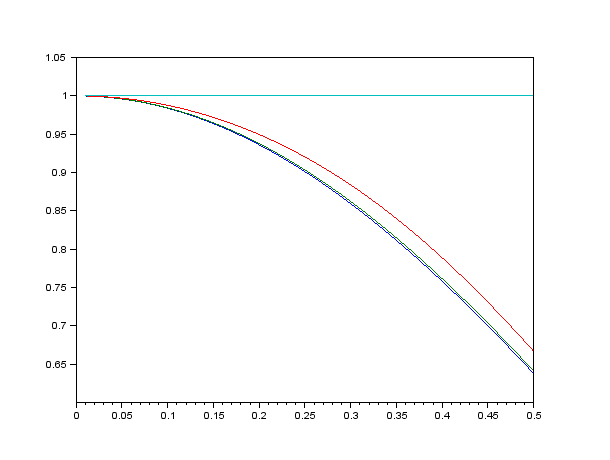
\includegraphics[scale=0.5]{img/graphe1.png}
\caption{courbe de $q(\alpha, G)$ pour $alpha \in \{0.1, 0.2, 0.5, 1\}$}
\end{figure}

\begin{itemize}
	\item 
A $\alpha$ fixé, quand $ \Delta t$ et $h$ tendent vers 0, $G$ tend vers 0. 
Et donc 
\begin{align*}
q(\alpha, G) 
&= \frac{\BigF{arcsin}{\alpha \pi G + \BigO{G^3} ) }}{\alpha \pi G} \\
&= \frac{\alpha \pi G  + \BigO{G^3} }{\alpha \pi G} \\
&= 1  + \BigO{G^2} \\
\end{align*}
On retrouve que le schéma est d'ordre 2.

	\item 
A $\alpha$ fixé, $G \to q(\alpha, G)$ est décroissante au voisinage de $0$. \textbf{Interpréation:} En prenant beaucoup de points par longueur d'onde,
la simulation colle mieux à la réalité.

	\item 
A $G$ fixé, $\alpha \to q(\alpha, G)$ est croissante, et tend vers $1$ en $\alpha \to 1$. Il vaut mieux prendre $\alpha = 1$.
	
	\item 
Prendre $\alpha \to 0$, ie $\Delta t =  \SmallO{h}$, revient à considérer une évolution continue en temps. On retrouve le schéma semi-discretisé. Formellement:
$ q(\alpha, G) \sim_{\alpha \to 0} \frac{sin(\pi G)}{\pi G}$ 
qui est le résultat trouvé à la question 3. 
Pour faire tendre $\alpha$ vers $0$, on a envie de laisser $h$ constant et faire tendre $\Delta t$ vers 0. Sauf qu'on vient de démontrer que dans ce cas là, la fonction de dispersion $q(\alpha, G) \approx sinc(\pi G)$ qui est décroissante en $h$


\end{itemize}




\subsubsection*{Passage à la 2D}
On modifie le schéma saute-mouton en conséquence. On pose $U^n_{i,j}$ comme approximation de $u(i \Delta x, j \Delta y, n \Delta t)$ 
où $\Delta x$ et $\Delta y$ les pas en espace dans les deux directions du plan $(\vec{x}, \vec{y})$. On propose le schéma suivant:

$$ \frac{1}{c^2} \frac{U^{n+1}_{i,j} - 2U^{n}_{i,j} + U^{n-1}_{i,j}}{\Delta t^2} - 
\frac{U^{n}_{i,j+1} - 2U^{n}_{i,j}+U^{n}_{i,j-1}}{\Delta x^2} 
-\frac{U^{n}_{i+1,j} - 2U^{n}_{i,j}+U^{n}_{i-1,j}}{\Delta y^2}
= 0$$
En cherchant les solutions de la forme:
$$ U^n_{\Delta x, \Delta y} = e^{i(w t^n - \vec{k} X_{\Delta x, \Delta y})} $$
où $\vec{k} . X_{\Delta x, \Delta y} = \Wrap{k_x i*\Delta x \, \vec{x} + k_y j*\Delta y \, \vec{y}}_{i, j} $, 
On trouve la relation de dispersion suivante:
$$ sin^2 \frac{w_{h, \Delta t} (k) t}{2} = \alpha_x ^ 2 sin^2 \frac{k_x \Delta x}{2} + \alpha_y ^ 2  sin^2 \frac{k_y \Delta y}{2} $$
où $\alpha_x = \frac{c \Delta t}{\Delta x}$ et  $ \alpha_y = \frac{c \Delta t}{\Delta y}$.

Si l'on prend $\Delta x = \Delta y = h$, la relation se simplifie en:
$$ sin^2 \frac{w_{h, \Delta t} (k) t}{2} = \alpha ^ 2 \Wrap{ sin^2 \frac{k_x h}{2} + sin^2 \frac{k_y h}{2} }$$

Cette équation en $w$ admet une solution si et seulement si 
$$\alpha ^ 2 sup_{\vec{k}} \left\{ sin^2 \frac{k_x \Delta x}{2} + sin^2 \frac{k_y \Delta y}{2} \right \} \leq 1$$
ie si $\alpha \leq \frac{\sqrt{2}}{2}$.

Pour trouver l'ordre du schéma, on procède comme précédemment:
Si $ 0 < \alpha < 1 $ et $ k \neq 0 $:
\begin{align*}
sin^2 \frac{w_{h, \Delta t} (k) \Delta t}{2} = \alpha ^ 2 \Wrap{sin^2 \frac{k_x h}{2} + sin^2 \frac{k_y h}{2}}
& \implies sin \frac{w_{h, \Delta t} (k) t}{2} = \pm \alpha  \sqrt{sin^2 \frac{k_x h}{2} + sin^2 \frac{k_y h}{2}}  \\
& \implies \frac{w_{h, \Delta t} (k)}{k c} = \pm \frac{ \BigF{arcsin}{\alpha  \sqrt{sin^2 \frac{k_x h}{2} + sin^2 \frac{k_y h}{2}} }}{ \alpha \frac{k h}{2} }\\
\end{align*}

Et donc:
\begin{align*}
\Wrap{ \frac{w_{h, \Delta t} (k)}{k c} }^2
&= \Wrap{\frac{\BigF{arcsin}{\alpha  \sqrt{sin^2 \frac{k_x h}{2} + sin^2 \frac{k_y h}{2}} }}{ \alpha \frac{k h}{2} } }^2 \\
\end{align*}
Si $\theta = arctan(\frac{ky}{kx})$, alors $cos(\theta) = \frac{ky}{k}$ et $sin(\theta) = \frac{kx}{k}$. Et donc:
$$ q(\alpha, G, \theta) = |\frac{w_{h,\Delta t}(k)}{kc}| 
= \frac{ \BigF{arcsin}{\alpha  \sqrt{sin^2(\pi G cos(\theta) )  + sin^2(\pi G sin(\theta) )} }}{ \alpha \pi G }$$

\begin{figure}
        \begin{subfigure}[b]{0.3\textwidth}
								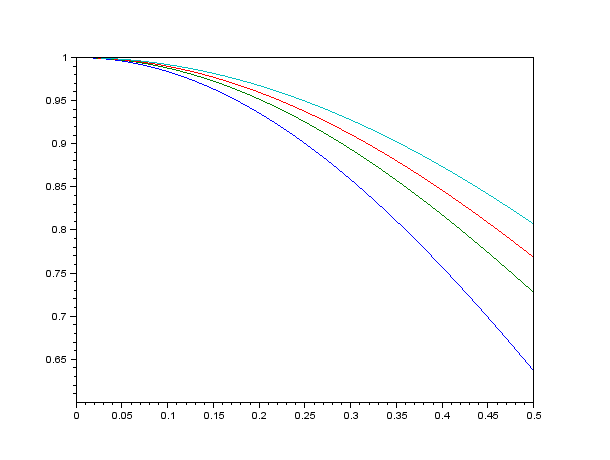
\includegraphics[scale=0.3]{img/graphe2-a.png}
                \caption{$\alpha = 0.01$}
        \end{subfigure}%
        ~
        \begin{subfigure}[b]{0.3\textwidth}
								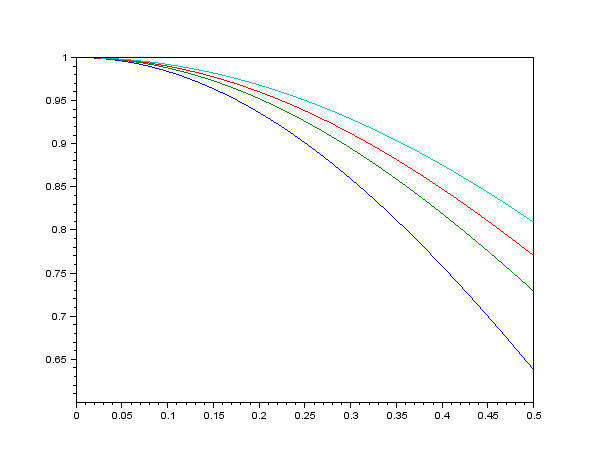
\includegraphics[scale=0.3]{img/graphe2-b.png}
                \caption{$\alpha = 0.1$}
        \end{subfigure}
				~
        \begin{subfigure}[b]{0.3\textwidth}
								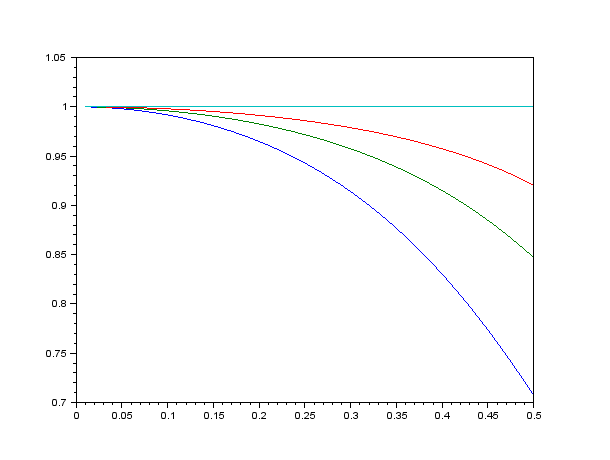
\includegraphics[scale=0.3]{img/graphe2-c.png}
                \caption{$\alpha = \frac{\sqrt 2}{2}$}
        \end{subfigure}
				\caption{Courbes de dispersion pour $\theta \in \{0, \frac{\pi}{8},  \frac{\pi}{6}, \frac{\pi}{4}\}$ }

\end{figure}


Le schéma présente des anisotropies parceque le coefficient de dispersion dépend de la direction de l'onde (paramétrée par $\theta$).
Contrairement au cas 1D, lorsque $\alpha = 1$, le schéma n'est plus exacte.

Le cas le plus favorable est le cas où $\theta = \frac{\pi}{4}$ et $\alpha = \frac{sqrt(2)}{2}$.  On obtient donc une solution exacte dans les directions diagonales.

Pour $\alpha$ fixé , $\theta \to q(\alpha, G, \theta)$ est symétrique par rapport à $\frac{\pi}{4}$, décroissante dans $[0, \frac{\pi}{4}]$
Le cas le plus défavorable est $\theta = 0$ ou $1$, ie dans le sens des directions du maillage.

\end{document}


